\chapter{Tools}
\vspace{6cm}
Developing this kind of systems is extremely complex, as can be seen from the above analysis, but it would be a lot harder without algorithms and libraries made by other people.
In order to make our solution clearer and honor their work, in the following paragraphs I will briefly describe all the tools used by our project.
\newpage

\section{Language}
Every algorithm is implemented in C++ and all the used libraries bindings are also in that same language because performance is a must for these situations.   

\section{Developing environment}
A common laptop with the following specifications:
\begin{itemize}
  \item A 2,5 GHz Intel core i7 processor
  \item 8gb of RAM
  \item Integrated graphic card
\end{itemize}
and Slackware Linux -current as Operating System.


\section{The camera}
\begin{figure}[hbt]
    \vspace{1cm}
    \centering
    \caption{The Playstation Eye}
    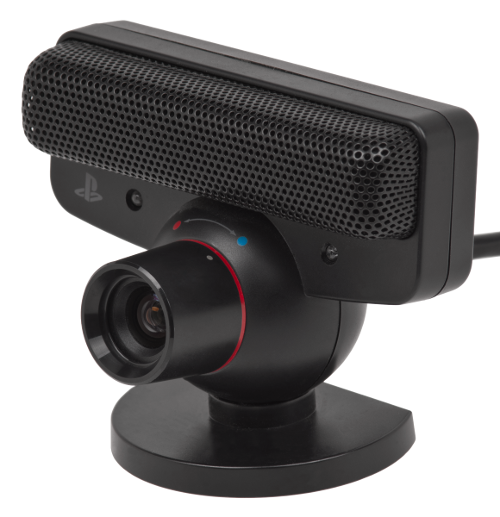
\includegraphics{img/pseye.png}
    \vspace{1cm}
\end{figure}

In order to stream videos or take pictures a Playstation 3 Eye has been used.
This camera can operate at 120Hz with a resolution of 320x240 pixels but we, instead, preferred to operate at 640x480 pixels with a frequency of 60Hz.
The device is automatically recognized and used without issues if the version of the Linux Kernel installed is later than the version 2.6.32 .
 

\section{Libraries}

\subsection{OpenCV}
This is the library which empower almost any device with a camera to process images and videos allowing manipulations with consolidated algorithms created by universities and companies in order to let the developer focus on their own solution of a problem.
In fact, OpenCV is the de facto standard for computer vision and it is wide-used in Sony Cameras for examples, but also on Android smartphones and iOS devices. 
\newline Used version: \textbf{2.4.9}

\subsection{ZBar}

The capability of decoding a QRCode is given by the ZBar library, which is open source and can decode also other kind of markers, for example: EAN-13/UPC-A, UPC-E, EAN-8 and Code 128.In addition, it is able to decode from a multitude of sources such as still images, raw intensity sensors and not only from video streams as the project shows. At the core of this possibility there is a streamlined implementation of the \textbf{ISO/IEC 18004:2000} encoding/decoding RFC in C which is perfect for embedded purposes.
\newline Used version: \textbf{0.10}.

\subsection{Eigen}
This library provide abstractions and utilities for linear algebra such as numerical solvers but also matrices and related algorithms which are the very one used by our project.
The whole code is free-software because it is licensed with MPLv2 and it is based on C++ templating system, in this way the developer can use only the needed header file which allows reasonable compilation time and flexibility.\cite{eigeninfo}
\newline Used version: \textbf{3.2.1}.

\section{Other algorithms}

\subsection{Rectification}
The rectification process removes the perspective and corrects distortion inside a picture by creating a new virtual image which contains every pixel from the first on their right position, minus pixels which goes out of the boundaries.
The new position of each pixel is found using linear transformation and adjusted with the focal length of the camera.
In order to simplify the concept, the following pseudo-code shows the general algorithm.

\vspace{1cm}
\begin{lstlisting}
void rectification(constant Camera c_real, Camera c_virtual)
{
    setupVirtualCamera(c_virtual);
    image_x_distortion_correction = linear_transformation(c_real.image.center.x,c_virtual.image.center.x);
    image_y_distortion_correction = linear_transformation(c_real.image.center.y,c_virtual.image.center.y);
    focal_correction = focal_distance(c_real.focal,c_virtual.focal);
    for (int i = 0; i < c_real.image.pixels.length ; i++)
    {
		
		oldX =  c_real.image.pixels[i].x
		            +image_x_distortion_correction
		            +focal_correction;
		oldY =  c_real.image.pixels[i].y
		            +image_y_distortion_correction
		            +focal_correction;
		
		/* compute the focal distance in order to find the point */
		newY = computeY(oldX,c_real.focal,c_virtual.focal);
		newX = computeX(oldY,c_real.focal,c_virtual.focal);
		
		if( isOutOfVirtualBound(newX,newY)) then continue;
		
		writePixel(c_virtual.image,
		     c_real.image.pixels[i],newX,newY);
		     
    }

}
\end{lstlisting}

\begin{figure}[hbt] 
    \centering
    \caption{before and after rectification}
    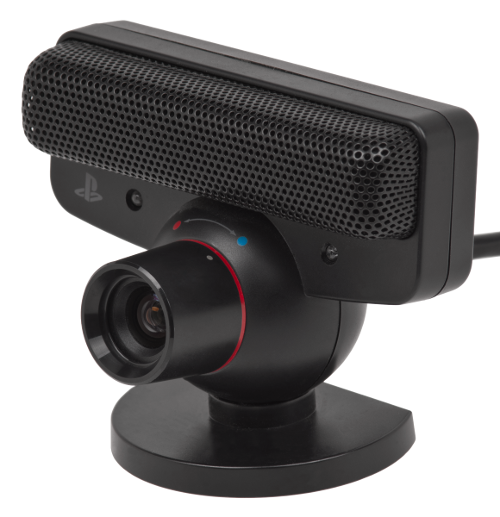
\includegraphics{img/pseye.png}
\end{figure}




 
